%\documentclass[dvipdfmx]{beamer}      % platex の場合
\documentclass[handout]{beamer}        % lualatex の場合
\usepackage{mySld}
\usepackage{multicol}

\begin{document}
\title{基礎コンピュータ工学\\第5章 機械語プログラミング\\(パート2)}
\date{}

\begin{frame}
  \titlepage
  \centerline{\url{https://github.com/tctsigemura/TecTextBook}}
  \vfill
  \centerline{本スライドの入手:
    \raisebox{-7mm}{
\includegraphics[scale=0.3]{../Img/QRs5_2.png}}}
\end{frame}

%==============================================================================
%\begin{frame}
%  \frametitle
%  \tableofcontents
%\end{frame}

\section{データ転送命令}
%==============================================================================
\begin{frame}
  \frametitle{データ転送命令}
  CPUとメモリの間でデータを転送する機械語命令(2種類)
  \begin{itemize}
  \item \texttt{LD(Load)命令}:CPUのレジスタ ← メモリ
  \item \texttt{ST(Store)命令}:メモリ ← CPUのレジスタ
  \end{itemize}
  \vfill
  \begin{minipage}{0.49\columnwidth}
  \centerline{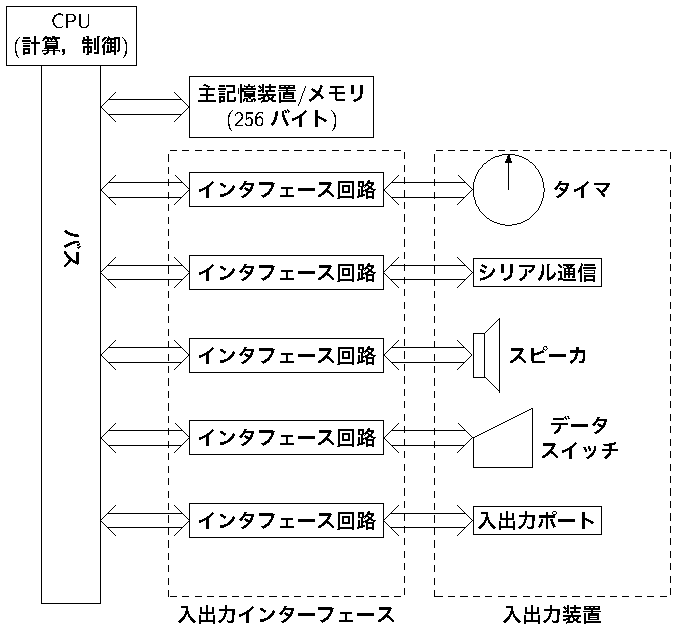
\includegraphics[scale=0.63,clip,trim=0 3cm 3cm 0]
    {../Tikz/kousei2.pdf}}
  \end{minipage}
  \begin{minipage}{0.49\columnwidth}
  \centerline{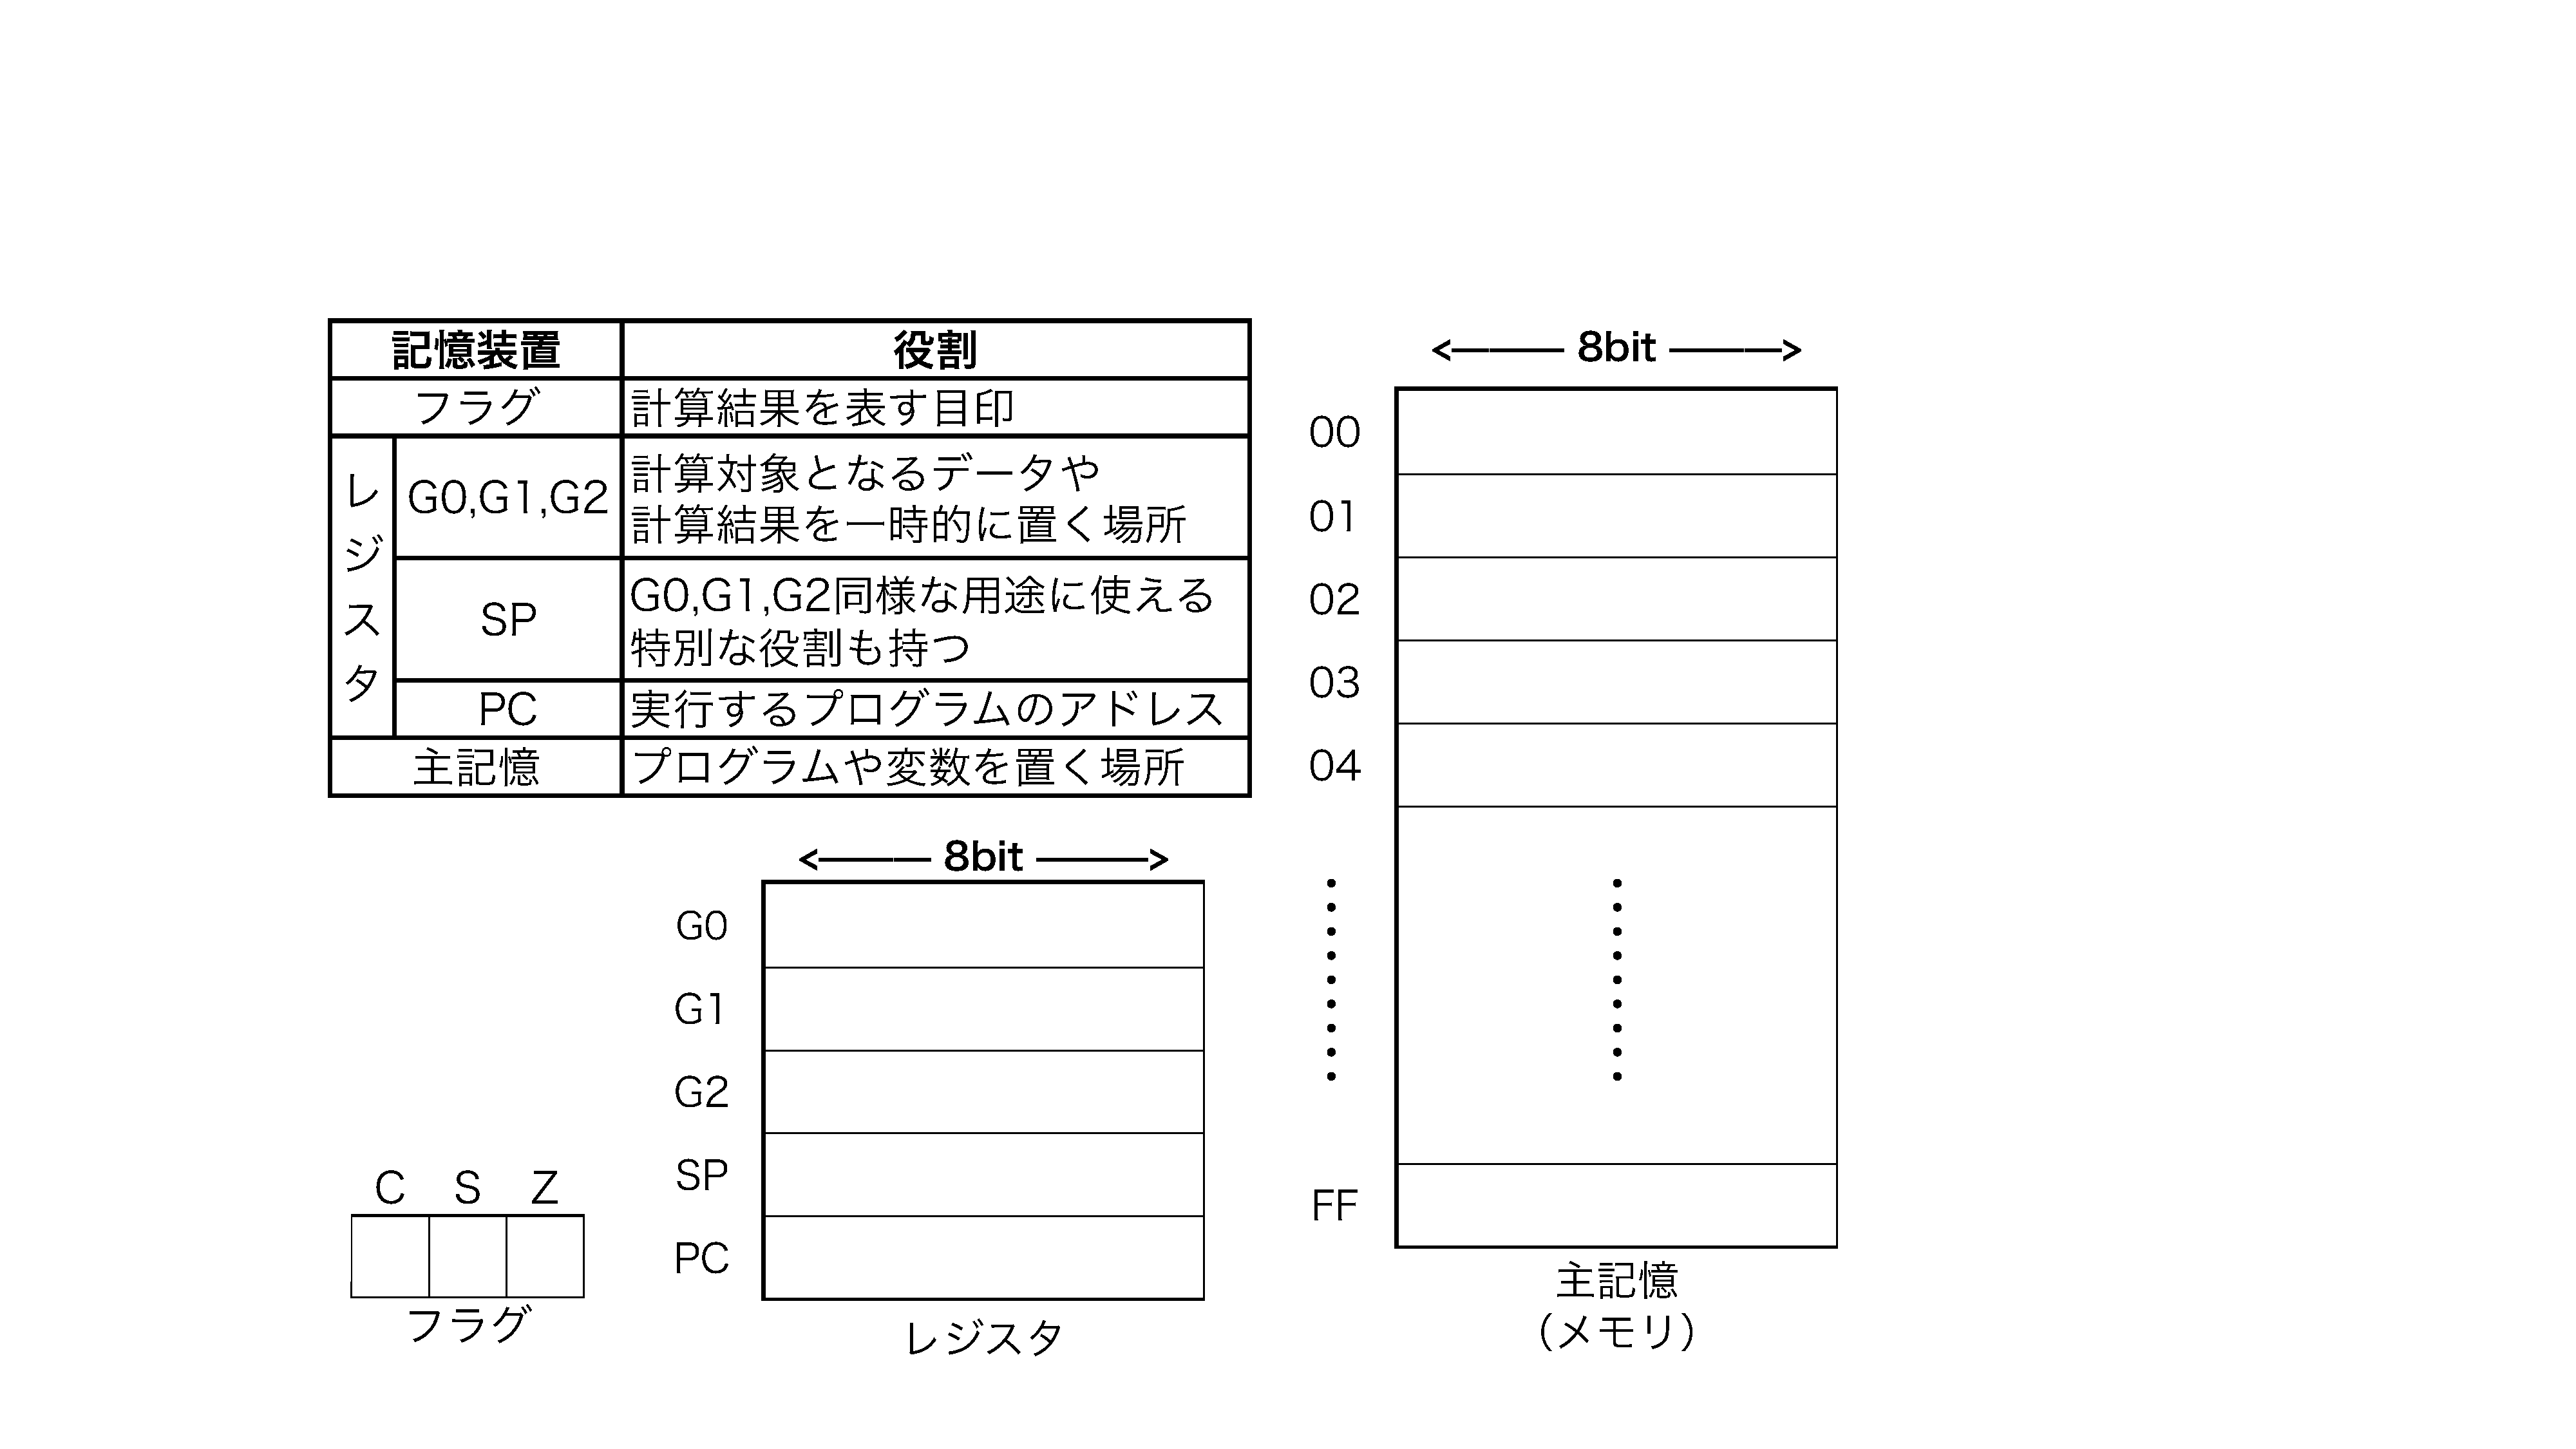
\includegraphics[scale=0.63,clip,trim=3cm 0 0 0]
    {../chap4/naibu.pdf}}
  \end{minipage}
\end{frame}

%==============================================================================
\begin{frame}
  \frametitle{LD(Load)命令(ニーモニックと命令フォーマット)}
  メモリ(\texttt{EA})からCPUのレジスタ(\texttt{GR})へ
  データを転送(コピー)する.

  \begin{description}
  \item[ニーモニック:] \texttt{LD GR,EA} ~~~~~~~~~ 例
    \vspace{0.5cm}

  \item[命令フォーマット:] 2バイトの長さを持つ.\\
    \twoByte{$0001_2$}{\GR~\XR}{\A}
  \item[フィールド:] \texttt{OP},\texttt{GR},\\ \texttt{XR},\texttt{A}

  \item[GRフィールドの意味と値:]GRの2ビットでCPUレジスタを指定する.\\
    {\small\begin{center}
      \begin{tabular}{c|c} \hline\hline
        GR & 意味 \\
        \hline
        $00_2$ & G0 \\
        $01_2$ & G1 \\
        $10_2$ & G2 \\
        $11_2$ & SP \\
      \end{tabular}
    \end{center}}

  \end{description}
\end{frame}

%==============================================================================
\begin{frame}
  \frametitle{LD(Load)命令(具体的な命令の例)}
  メモリの3番地からからG1レジスタへデータを転送(コピー)する.

  \begin{description}
  \item[ニーモニック:] \texttt{LD G1,03H}

  \item[命令フォーマット:] G1と03Hを反映する.\\
    \twoByte{$0001_2$}{$01_2$~$00_2$}{$0000~0011_2$}
    \vspace{1.0cm}

  \item[メモリに格納した状態:]\texttt{HALT}命令やデータも格納している.
    {\ttfamily\small\begin{center}
      \begin{tabular}{c|c|l}
        \multicolumn{1}{c}{番地} &
        \multicolumn{1}{c}{命令} &
        \multicolumn{1}{c}{}  \\
        \cline{2-2}
        $00_{16}$ & $14_{16}$ & LD G1,03H  \\
        \cline{2-2}
        $01_{16}$ & $03_{16}$ &            \\
        \cline{2-2}
        $02_{16}$ & $FF_{16}$ & HALT       \\
        \cline{2-2}
        $03_{16}$ & $12_{16}$ & 何かデータ \\
        \cline{2-2}
      \end{tabular}
    \end{center}}
  \end{description}
\end{frame}

%==============================================================================
\begin{frame}
  \frametitle{LD(Load)命令(少し長い例)}
  \begin{description}
  \item[プログラムの例:] データを \texttt{G0},\texttt{G1} にロードする.\\
    {\ttfamily\small\begin{center}
      \begin{tabular}{|l|l|l|l l|} \hline
        番地 & 機械語 & ラベル & \multicolumn{2}{|c|}{ニーモニック} \\
        \hline
        $00_{16}$ & $10_{16}$ $05_{16}$ & & LD   & G0,05H \\
        $02_{16}$ & $14_{16}$ $06_{16}$ & & LD   & G1,06H \\
        $04_{16}$ & $FF_{16}$           & & HALT &       \\
        \hline
      \end{tabular}
    \end{center}}
    \vfill

    \item[メモリに格納した状態:] 何かデータも準備する必要がある.
      {\ttfamily\small\begin{center}
        \begin{tabular}{r|c|l}
          \multicolumn{1}{c}{番地} &
          \multicolumn{1}{c}{機械語} &
          \multicolumn{1}{c}{意味} \\
          \cline{2-2}
          $00_{16}$ & $10_{16}$ & LD G0,05H \\
          \cline{2-2}
          $01_{16}$ & $05_{16}$ &           \\
          \cline{2-2}
          $02_{16}$ & $14_{16}$ & LD G1,06H \\
          \cline{2-2}
          $03_{16}$ & $06_{16}$ &           \\
          \cline{2-2}
          $04_{16}$ & $FF_{16}$ & HALT      \\
          \cline{2-2}
          $05_{16}$ & $12_{16}$ & データ!!\\
          \cline{2-2}
          $06_{16}$ & $34_{16}$ & データ!!\\
          \cline{2-2}
        \end{tabular}
      \end{center}}
      \vfill

  \end{description}
\end{frame}

%==============================================================================
\begin{frame}
  \frametitle{LD(Load)命令(フローチャートの描き方)}
  \begin{description}
  \item[LD命令のフローチャート:] \texttt{[}と\texttt{]}を忘れないように!\\
    \centerline{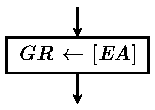
\includegraphics[scale=0.8]{../Tikz/ld.pdf}}
    \vfill
    
  \item[LD命令のフローチャート例:]
    \texttt{START}と\texttt{END}を追加 \\
    \centerline{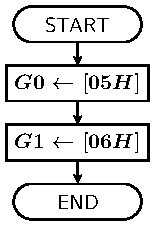
\includegraphics[scale=0.8]{../Tikz/lds.pdf}}
    \vfill

  \end{description}
\end{frame}

%==============================================================================
\begin{frame}
  \frametitle{ST(Store)命令(ニーモニックと命令フォーマット)}
  CPUのレジスタからメモリへデータを転送(コピー)する.
  \begin{description}
  \item[ニーモニック:] \texttt{ST GR,EA}
    \vspace{0.5cm}
  \item[命令フォーマット:] 2バイトの長さを持つ.\\
    \twoByte{$0010_2$}{\GR~\XR}{\A}
    \vspace{1.0cm}
  \item[ST命令のフローチャート:] \texttt{[}と\texttt{]}を忘れないように!\\
    \centerline{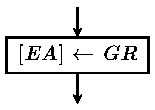
\includegraphics[scale=0.8]{../Tikz/st.pdf}}
    \vfill
  \end{description}
\end{frame}

%==============================================================================
\begin{frame}
  \frametitle{ST(Store)命令(プログラム例)}
  \begin{description}
  \item[プログラムの例:]
    \texttt{05H}番地のデータを\texttt{06H}番地にコピーする.
    {\ttfamily\small\begin{center}
      \begin{tabular}{|l|l|l|l l|} \hline
        番地 & 機械語 & ラベル & \multicolumn{2}{|c|}{ニーモニック} \\
        \hline
        00 & 10 05 & & LD   & G0,05H \\
        02 & 20 06 & & ST   & G0,06H\\
        04 & FF    & & HALT & \\
        \hline
      \end{tabular}
    \end{center}}
    {\footnotesize 番地と機械語はいつも16進数で書く(小さく16と書く必要なし).}
  \item[フローチャート:] 上のプログラムのフローチャートを描いてみる.
    \vfill
  \end{description}
  \vfill
  \vfill
  \vfill
\end{frame}

%==============================================================================
\begin{frame}
  \frametitle{演習}
  次の手順を守って演習を行う.
  \begin{enumerate}
  \item[1.] フローチャートを描いて考えをまとめる.
  \item[2.] ニーモニック(オペレーション,オペランド)に変換する.
  \item[3.] 番地(アドレス)を決める.
  \item[4.] 機械語を決める.
  \item[5.] TeCに打ち込み実行して結果を確認する.
  \end{enumerate}
  \centerline{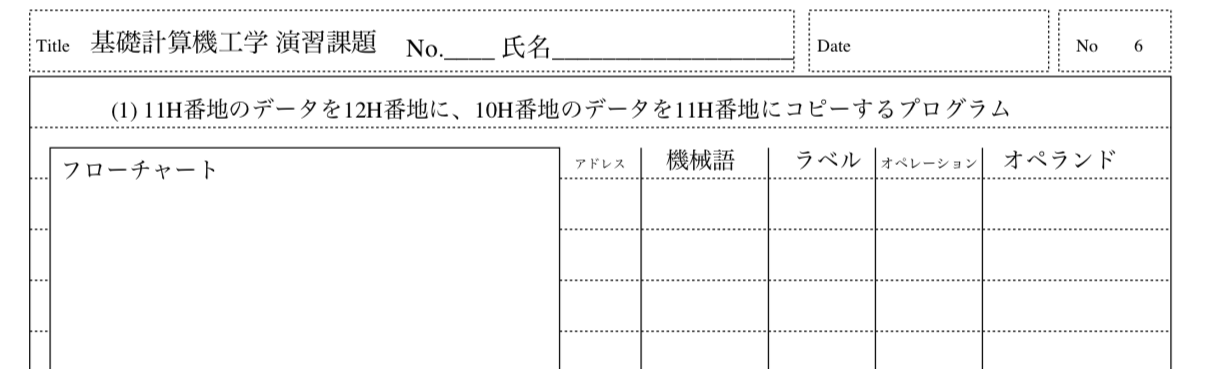
\includegraphics[scale=0.5]{tejyun.png}}
  \vfill
  \vfill
\end{frame}

%==============================================================================
%\begin{frame}
%  \frametitle{}
%\end{frame}

\end{document}
